\documentclass{article}
\usepackage[utf8]{inputenc}
\usepackage{tikz}
\usepackage{xcolor}
\pagecolor{white}

\begin{document}

\begin{tikzpicture}
\draw (0,0) -- (6,0);
\end{tikzpicture}

\bigskip

\begin{tikzpicture}
\draw (0,0) -- (6,0) -- (6,6) -- (0,6) -- cycle;
\end{tikzpicture}

\bigskip

\begin{tikzpicture}
\draw (0,0) rectangle (6,6);
\draw (0,0) parabola (6,6);
\end{tikzpicture}

\bigskip

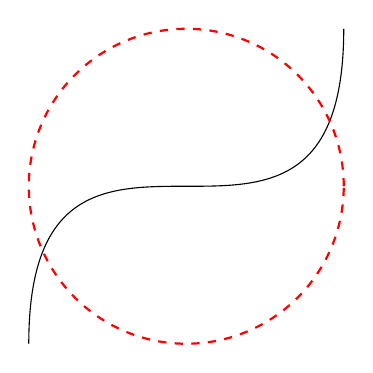
\begin{tikzpicture}
\draw (0,0) .. controls (0,4) and (4,0) .. (4,4);
\draw[red,thick,dashed] (2,2) circle (2cm);
\end{tikzpicture}

\bigskip

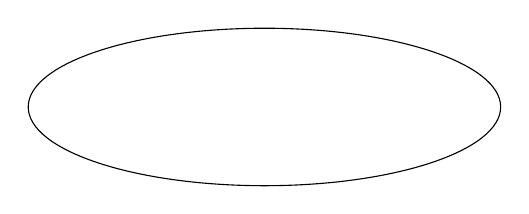
\begin{tikzpicture}
\draw (2,2) ellipse (3cm and 1cm);
\end{tikzpicture}

\bigskip

\begin{tikzpicture}
\draw (3,0) arc (0:160:3cm);
\end{tikzpicture}

\bigskip

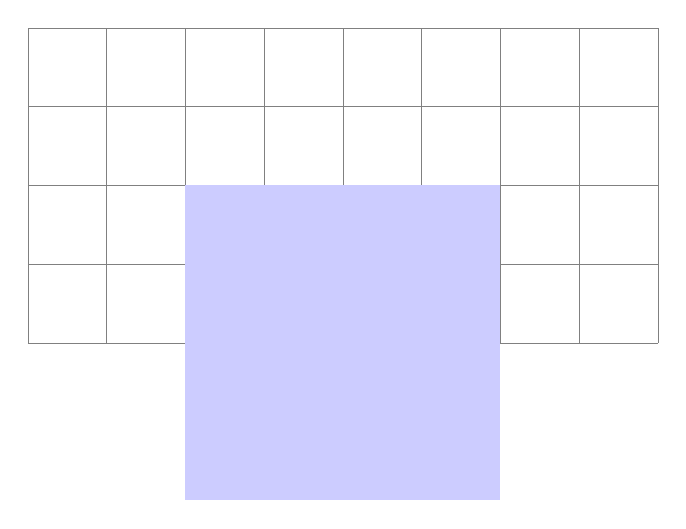
\begin{tikzpicture}
\draw[step=1cm,gray,very thin] (-2,2) grid (6,6);
\fill[blue!20!white] (0,0) rectangle (4,4);
\end{tikzpicture}

\bigskip

\begin{tikzpicture}
\draw[step=1cm,gray,very thin] (-1.9,-1.9) grid (5.9,5.9);
\end{tikzpicture}

\bigskip

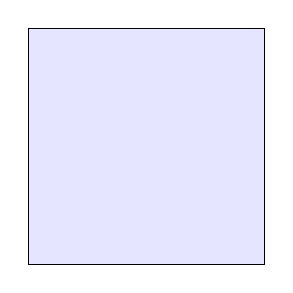
\begin{tikzpicture}
\filldraw[fill=blue!10!white, draw=black] (0,0) rectangle (3,3);
\end{tikzpicture}

\bigskip


\begin{tikzpicture}
\shade[left color=yellow, right color=red] (0,0) rectangle (6,6);
\end{tikzpicture}

\bigskip


\begin{tikzpicture}
\shade[top color=blue, bottom color=green] (0,0) rectangle (6,6);
\end{tikzpicture}

\bigskip

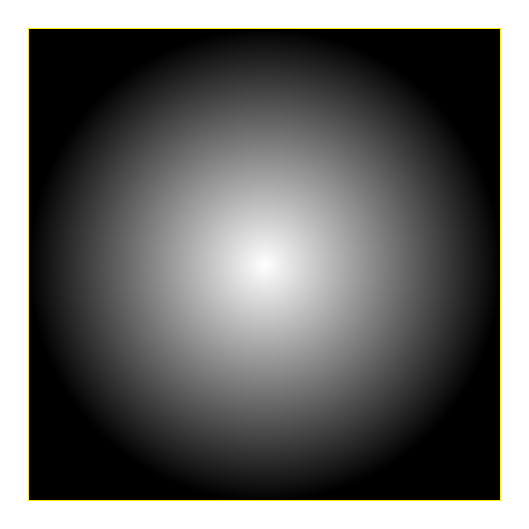
\begin{tikzpicture}
\shadedraw[inner color=white, outer color=black, draw=yellow] (0,0) rectangle (6,6);
\end{tikzpicture}

\bigskip

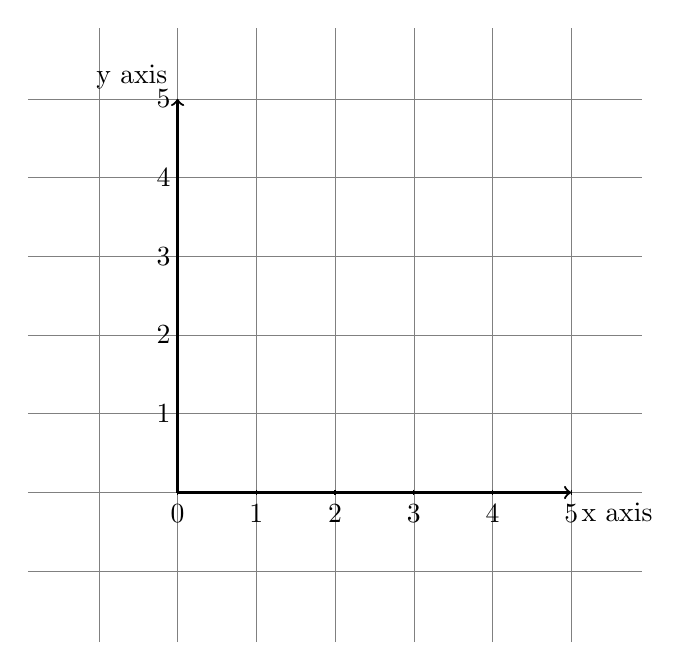
\begin{tikzpicture}
\draw[step=1cm,gray,very thin] (-1.9,-1.9) grid (5.9,5.9);
\draw[thick, ->] (0,0) -- (5,0) node[anchor=north west] {x axis};
\draw[thick, ->] (0,0) -- (0, 5) node[anchor=south east] {y axis};

\foreach \x in {0,1,2,3,4,5}
	\draw (\x cm, 1pt) -- (\x cm, -1pt) node[anchor=north] {$\x$};
\foreach \y in {1,2,3,4,5}
	\draw (1pt, \y cm) -- (1pt, \y cm) node[anchor=east] {$\y$};
\end{tikzpicture}


















\end{document}